\chapter{黑洞熵、全息性与德西特空间}

\lectureoverview{我们完成上一讲开始的那个对应关系论证。高度激发的弦具有正比于其质量的熵，而施瓦茨席尔德黑洞具有正比于其面积的熵。这两个公式之间的联系，并不是通过把一个强引力黑洞等同于一条自由弦而建立的，而是通过缓慢改变弦耦合，直到两种描述相遇。面积定律于是自然地导向全息原理，而本讲的最后一部分引入膨胀空间以及德西特几何，其视界将在下一讲研究。}

\section{回到计数问题}

长弦计数中还有一个未了结之处。如果把一个固定的总长度分配给若干条弦，那么长度相同的全同弦是不可区分的。然而它们在盒子中的位置仍然是态的一部分，而盒子的尺寸被选为大致等于相应的单条长弦所占据的大小。

\begin{classroomqa}
\audiencequestion{这些短弦彼此可区分吗，它们的位置要计入吗？\lecturetimestamp{00:00:37}}
\lecturerresponse{性质全同的弦是不可区分的，但它们在盒子中的位置要计入。比较是在固定体积下进行的，该体积被选为与长弦所占据的区域相匹配。}
\end{classroomqa}

这一点确定之后，我们就可以陈述目标了。我们将汇集一个简短的方程清单，并用它们得到黑洞熵的标度关系。不需要积分或无穷求和。困难不在于代数；困难在于知道哪些量可以比较，以及在论证的哪个阶段进行比较。

\section{自然单位与普朗克面积}

令
\begin{equation}
c=\hbar=1,
\label{eq:l07-natural-units}
\end{equation}
但保持牛顿常数显式出现。第一个推论是时间和长度具有相同的单位。光子关系式
\begin{equation}
E=\frac{\hbar c}{\lambda}
\end{equation}
以及质能关系 \(E=mc^2\) 于是给出
\begin{equation}
[M]=L^{-1}.
\label{eq:l07-mass-dimension}
\end{equation}
因此质量可以表示为长度的倒数。

\begin{figure}[htbp]
\centering
\includegraphics[width=0.62\textwidth]{lecture_07_figure_02.png}
\caption{量纲论证开始时采用的自然单位约定。能量公式已在上面的方程中补全。}
\lectureframe{00:03:27.900}
\end{figure}

要确定 \(G_N\) 的单位，只需把牛顿加速度用作量纲记账：
\begin{equation}
a\sim\frac{G_NM}{R^2}.
\end{equation}
因为 \(T\) 和 \(L\) 具有相同的单位，所以 \([a]=L/T^2=L^{-1}\)。结合方程~\eqref{eq:l07-mass-dimension}，这给出
\begin{equation}
[G_N]=L^2.
\end{equation}
在这些单位下，牛顿常数是一个面积。通过
\begin{equation}
G_N=\ell_p^2,
\label{eq:l07-planck-area}
\end{equation}
定义普朗克长度，我们立刻明白为什么 \(A/G_N=A/\ell_p^2\) 是无量纲的：它度量的是以普朗克面积计的面积。

\section{弦耦合与引力的强度}

现在必须把引力翻译成弦的语言。有用的图像是交换过程。当一条弦与自身相交时，它可以分裂并重新连接。一个小闭弦圈可以由一个物体发射并被另一个物体吸收；当该激发是引力子时，这个过程就传递引力。发射时出现一个相互作用因子，吸收时又出现一个，因此交换强度中含有 \(g_s^2\)。

耦合 \(g_s\) 是无量纲的。更准确地说，它是振幅层面的耦合，而概率或速率从 \(g_s^2\) 阶开始。\editorialnote{本讲有时把 \(g_s\) 称为概率，随后又更正为概率的平方根。微扰耦合属于振幅层面。} 由于 \(G_N\) 具有面积的量纲，仍然缺少一个长度标度。基本弦长 \(\ell_s\)，即一次基本弦振动的尺度，提供了它：
\begin{equation}
G_N\sim g_s^2\ell_s^2,
\qquad
\ell_p\sim g_s\ell_s.
\label{eq:l07-planck-string}
\end{equation}

\begin{figure}[htbp]
\centering
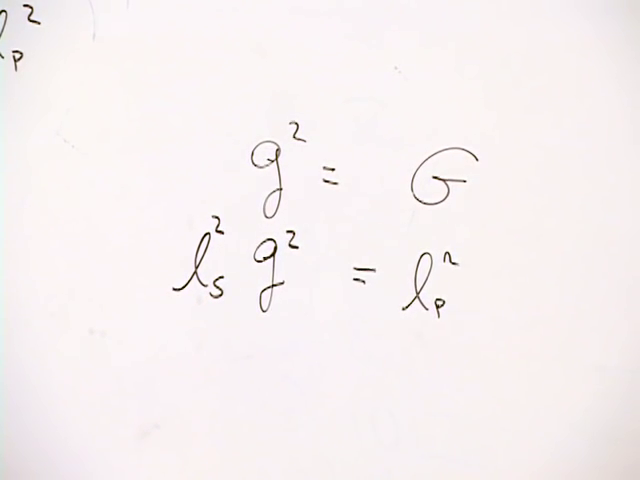
\includegraphics[width=0.72\textwidth]{lecture_07_figure_05.png}
\caption{黑板上的耦合关系：\(G_N=\ell_p^2\) 和 \(g_s^2\ell_s^2\sim\ell_p^2\)。}
\lectureframe{00:12:15.000}
\end{figure}

在弱耦合下，\(g_s\ll1\)，普朗克长度远小于弦长。把 \(g_s\) 调小会削弱引力，同时使基本弦标度保持不变。\editorialnote{对于有效的四维理论，紧致化数据和数值约定也会进入 \(G_N\)。它们被保持固定，并在这个标度论证中被略去。}

\section{计数一条长弦}

熵计数的是指定一个态所需的基本决定。把一条高度激发的弦替换为在正方形点阵上的行走。在每个顶点，下一段连线可以指向四个方向之一。无论这个基本选择被描述为一次四向决定还是两次二元决定，改变的只是一个量级为一的常数。重要的是步数。

如果\(L\)是弦的轮廓长度，而每一步的长度为\(\ell_s\)，那么需要
\begin{equation}
N=\frac{L}{\ell_s}
\end{equation}
步。行走的数目呈指数增长，示意性地为\(\Omega_N\sim q^N\)，其中\(q\)为1阶量，因此
\begin{equation}
S_{\mathrm{str}}=\log\Omega_N\sim N\sim\frac{L}{\ell_s}.
\label{eq:l07-string-entropy-length}
\end{equation}

\begin{figure}[htbp]
\centering
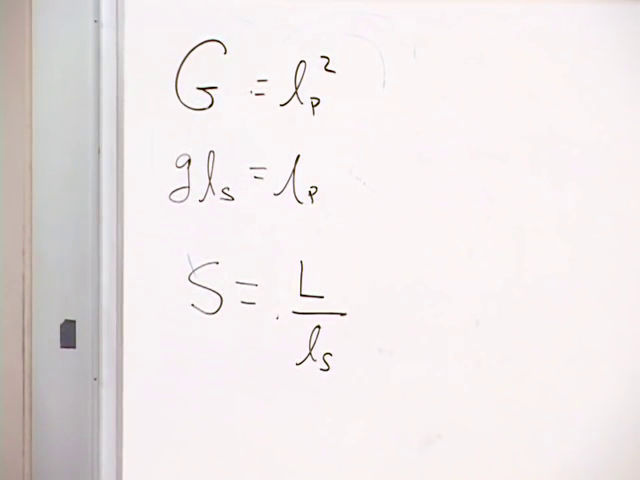
\includegraphics[width=0.68\textwidth]{lecture_07_figure_03.png}

\vspace{0.7em}
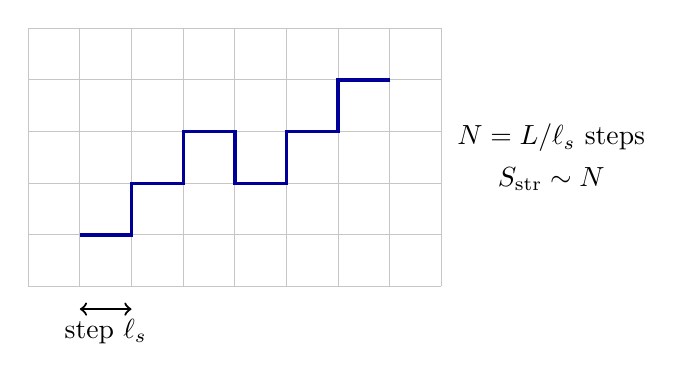
\begin{tikzpicture}[scale=0.82]
  \draw[step=0.8cm,gray!45,thin] (0,0) grid (6.4,4.0);
  \draw[very thick,blue!60!black]
    (0.8,0.8)--(1.6,0.8)--(1.6,1.6)--(2.4,1.6)--(2.4,2.4)--
    (3.2,2.4)--(3.2,1.6)--(4.0,1.6)--(4.0,2.4)--(4.8,2.4)--
    (4.8,3.2)--(5.6,3.2);
  \draw[<->,thick] (0.8,-0.35)--(1.6,-0.35);
  \node[below] at (1.2,-0.35) {step \(\ell_s\)};
  \node[align=center] at (8.1,2.0) {\(N=L/\ell_s\) steps\\[0.3em]\(S_{\mathrm{str}}\sim N\)};
\end{tikzpicture}
\caption{黑板上的点阵模型及其整理后的随机行走解释。决定选择数目的是轮廓长度，而不是缠结球的直径。}
\lectureframe{00:17:20.000}
\end{figure}

质量由同样的基本线段来计数。长度为\(\ell_s\)的线段具有质量标度
\begin{equation}
m_{\mathrm{seg}}\sim\frac{1}{\ell_s}.
\end{equation}

\begin{classroomqa}
\audiencequestion{基本线段被赋予长度\(\ell_s\)吗？\lecturetimestamp{00:18:56}}
\lecturerresponse{是的。它的特征长度为\(\ell_s\)，因此在自然单位下其特征质量为\(1/\ell_s\)。}
\end{classroomqa}

将\(L/\ell_s\)个线段的质量相加得到
\begin{equation}
M\sim\frac{L}{\ell_s}\frac{1}{\ell_s}
=\frac{L}{\ell_s^2},
\qquad
L\sim M\ell_s^2.
\label{eq:l07-string-mass}
\end{equation}
振荡弦的动能和势能已被压缩进这个标度关系；详细的统计力学处理给出相同的依赖关系。代入方程~\eqref{eq:l07-string-entropy-length}便得到我们所需的弦公式：
\begin{equation}
S_{\mathrm{str}}\sim M\ell_s.
\label{eq:l07-string-entropy-mass}
\end{equation}

\begin{figure}[htbp]
\centering
\includegraphics[width=0.66\textwidth]{lecture_07_figure_04.png}
\caption{比较之前所汇总的弦一侧各列：\(\ell_p\sim g_s\ell_s\)、\(S_{\mathrm{str}}\sim L/\ell_s\sim M\ell_s\)和\(M\sim L/\ell_s^2\)。}
\lectureframe{00:21:57.800}
\end{figure}

\section{为什么自由弦还不是黑洞}

在引力一侧，精确的半经典公式为
\begin{equation}
S_{\mathrm{BH}}=\frac{A}{4G_N}.
\label{eq:l07-bh-exact}
\end{equation}

\begin{classroomqa}
\audiencequestion{分母中应取什么数值系数？\lecturetimestamp{00:23:28}}
\lecturerresponse{4。对应论证将恢复标度关系，但过于粗糙，无法确定那个精确因子。}
\end{classroomqa}

对于四维施瓦茨席尔德黑洞，
\begin{equation}
R_s=2G_NM,
\qquad
A=4\pi R_s^2.
\end{equation}
如讲座所做的那样略去数值常数，
\begin{align}
S_{\mathrm{BH}}
&\sim\frac{A}{G_N}
\sim\frac{(G_NM)^2}{G_N} \\
&\sim M^2G_N
\sim M^2\ell_p^2.
\label{eq:l07-bh-scaling}
\end{align}

\begin{figure}[htbp]
\centering
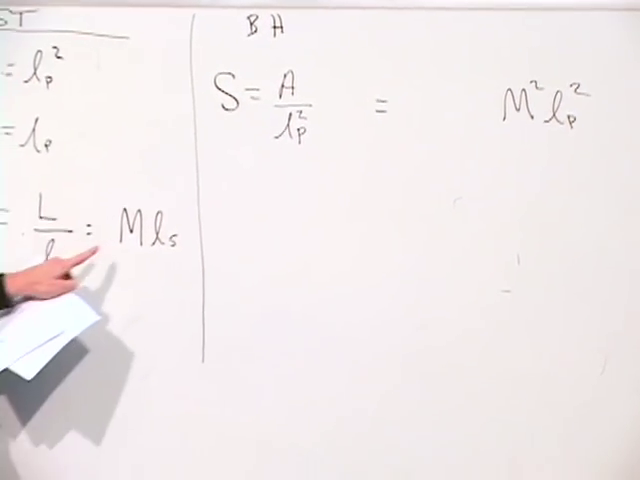
\includegraphics[width=0.72\textwidth]{lecture_07_figure_06.png}
\caption{黑板上完成的比较：弦熵是以弦单位为单位的长度，而黑洞熵是以普朗克单位为单位的面积。}
\lectureframe{00:25:35.000}
\end{figure}

方程~\eqref{eq:l07-string-entropy-mass}与\eqref{eq:l07-bh-scaling}之间的相似性具有启发性，但它们并非同一个公式。简单地把原来的黑洞称为自由弦并代入，是错误的。自由弦计数忽略了弦各部分之间的吸引相互作用，而正是这种相互作用把弦压缩成黑洞，并通过负结合能降低其总能量。

恒星使这一错误变得熟悉。把恒星质量的热气体放入一个过大的盒子中，并不是恒星的模型，即使温度相同。自引力会改变平衡尺寸以及能量与熵之间的关系。追踪长弦的每一个自相互作用会很困难，因此我们将避免这样做。

\begin{classroomqa}
\audiencequestion{如果一个小环从长弦上离开，它的熵会减少。那么引力子交换是否因此降低引力系统的熵？\lecturetimestamp{00:28:48}}
\lecturerresponse{在此处所使用的平衡交换过程中并非如此。虚激发沿两个方向发射和吸收；这幅漫画并不是永久失去一个弦片段的字面过程。它目前唯一的目的是确定两个耦合因子，从而确定\(g_s^2\)依赖关系。}
\end{classroomqa}

\section{绝热对应游戏}

不如从引力可忽略之处开始。当\(g_s\to0\)时，弦相互交叉而不分裂或合并，自引力吸引消失。增大\(g_s\)，同时保持\(\ell_s\)固定：引力增强，高度激发的弦收缩，最终变成黑洞。缓慢反向转动旋钮，黑洞必须回到弦态。它可能变成少量长弦，但上一讲的高能计数表明，主导扇区包含一根长弦，而不是由大量短弦组成的气体。

\begin{classroomqa}
\audiencequestion{改变耦合时保持什么固定？\lecturetimestamp{00:32:19}}
\lecturerresponse{弦长\(\ell_s\)，因而基本弦质量标度\(1/\ell_s\)，保持固定。旋钮改变\(g_s\)，从而改变\(G_N\sim g_s^2\ell_s^2\)。}
\end{classroomqa}

变化必须是缓慢、孤立且可逆的。在这些条件下，熵是绝热不变量：
\begin{equation}
\Delta S=0.
\label{eq:l07-adiabatic}
\end{equation}
如果发生耗散或不受控的跃迁，仅靠缓慢是不够的。这里``绝热''意味着同一族态可以被连续追踪。\editorialnote{这是绝热一词的可逆热力学含义。不可逆过程可以在无热流的意义上是绝热的，却仍然产生熵。}

设目标黑洞的质量为 \(M_0\)，耦合为 \(g_{s,0}\)。在使用我们试图解释的面积公式之前，量纲分析只能说明：一个中性、不旋转黑洞的熵是如下无量纲组合的某个函数
\begin{equation}
S_{\mathrm{BH}}=f(M\ell_p)
=f(Mg_s\ell_s).
\label{eq:l07-entropy-function}
\end{equation}
在 \(\ell_s\) 固定时，一条等熵路径因此保持
\begin{equation}
Mg_s=M_0g_{s,0}
\label{eq:l07-adiabat}
\end{equation}
不变，前提是沿着同一支态进行。

随着 \(g_s\) 减小，负结合能被移除，因此质量 \(M\) 沿此路径上升。底层的弦构型也变得更松散并延展开来。然而，形式上的施瓦茨席尔德半径在绝热线上表现为 \(R_s\sim Mg_s^2\ell_s^2\sim g_s\ell_s\)，因此反而减小。\editorialnote{口头讨论中用 ``增长'' 来描述从引力束缚中释放出来的物体。不应将其理解为施瓦茨席尔德半径沿所导出的绝热线增长。}

\begin{classroomqa}
\audiencequestion{当引力被减弱时，该物体是增长还是收缩？\lecturetimestamp{00:36:28}}
\lecturerresponse{它的弦结构被释放并膨胀，而它的质量增加，因为负结合能被移除。由黑洞公式给出的半径减小，直到达到弦尺度，在那里这种黑洞描述不再有用。}
\end{classroomqa}

\section{两条曲线及其交点}

纵轴为质量，横轴为弦耦合。方程~\eqref{eq:l07-adiabat} 是一条双曲线，\(M\propto g_s^{-1}\)。

\begin{classroomqa}
\audiencequestion{乘积 \(Mg_s\) 为常数的曲线是什么类型？\lecturetimestamp{00:44:08}}
\lecturerresponse{一条双曲线。它是通过目标点 \((g_{s,0},M_0)\) 的绝热线。}
\end{classroomqa}

第二条曲线标志着两种描述之间的过渡。一旦黑洞的半径小于基本弦的涨落尺度，它就不能被分辨为传统的施瓦茨席尔德几何。因此我们通过下式估计对应点
\begin{equation}
R_s\sim\ell_s.
\label{eq:l07-correspondence-radius}
\end{equation}
利用 \(R_s\sim MG_N\) 和方程~\eqref{eq:l07-planck-string}，这变为
\begin{equation}
Mg_s^2\ell_s^2\sim\ell_s,
\qquad
Mg_s^2\sim\frac{1}{\ell_s}.
\label{eq:l07-transition-curve}
\end{equation}
因此过渡曲线按 \(M\propto g_s^{-2}\) 下降，比绝热线更陡。

\begin{figure}[htbp]
\centering
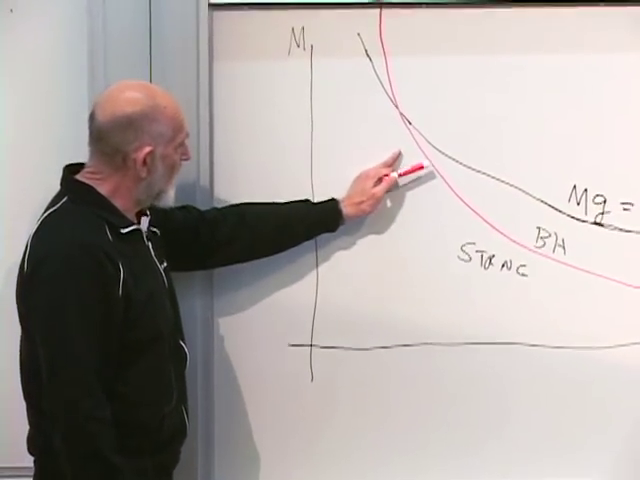
\includegraphics[width=0.70\textwidth]{lecture_07_figure_07.png}

\vspace{0.6em}
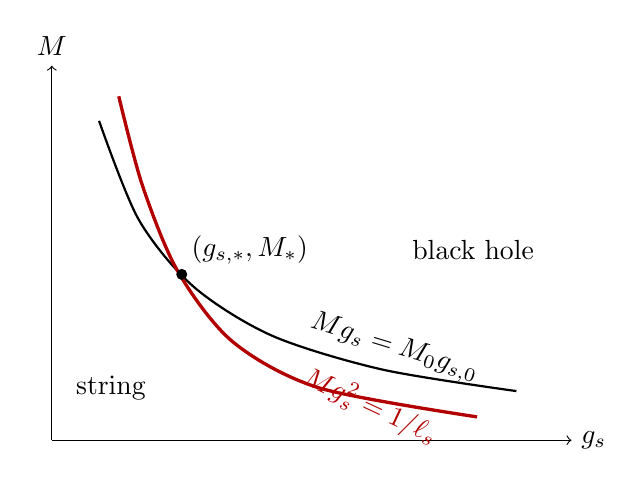
\begin{tikzpicture}[x=1cm,y=0.78cm]
  \draw[->] (0.4,0.4)--(7.0,0.4) node[right] {\(g_s\)};
  \draw[->] (0.4,0.4)--(0.4,6.5) node[above] {\(M\)};
  \draw[thick,black] plot[smooth] coordinates {(1.0,5.6) (1.5,4.0) (2.2,2.9) (3.2,2.1) (4.6,1.55) (6.3,1.2)};
  \draw[very thick,red!70!black] plot[smooth] coordinates {(1.25,6.0) (1.55,4.55) (2.0,3.15) (2.7,2.0) (3.8,1.25) (5.8,0.78)};
  \fill (2.05,3.1) circle (2pt) node[above right] {\((g_{s,*},M_*)\)};
  \node[black,rotate=-17] at (4.75,1.9) {\(Mg_s=M_0g_{s,0}\)};
  \node[red!70!black,rotate=-25] at (4.45,0.95) {\(Mg_s^2=1/\ell_s\)};
  \node at (5.75,3.5) {black hole};
  \node at (1.15,1.25) {string};
\end{tikzpicture}
\caption{黑板上的图及其整理后的解释。黑色绝热线与更陡的红色对应曲线相交于物体变为弦状的点。}
\lectureframe{00:49:35.000}
\end{figure}

在交点 \((M_*,g_{s,*})\) 处，两个方程为
\begin{align}
M_*g_{s,*} &= M_0g_{s,0}, \\
M_*g_{s,*}^2 &\sim \frac{1}{\ell_s}.
\end{align}
将第一个方程平方并除以第二个方程：
\begin{equation}
M_*
\sim M_0^2g_{s,0}^2\ell_s.
\end{equation}
乘以 \(\ell_s\)，
\begin{equation}
M_*\ell_s
\sim M_0^2g_{s,0}^2\ell_s^2
\sim M_0^2G_{N,0}.
\label{eq:l07-crossover-result}
\end{equation}

\begin{figure}[htbp]
\centering
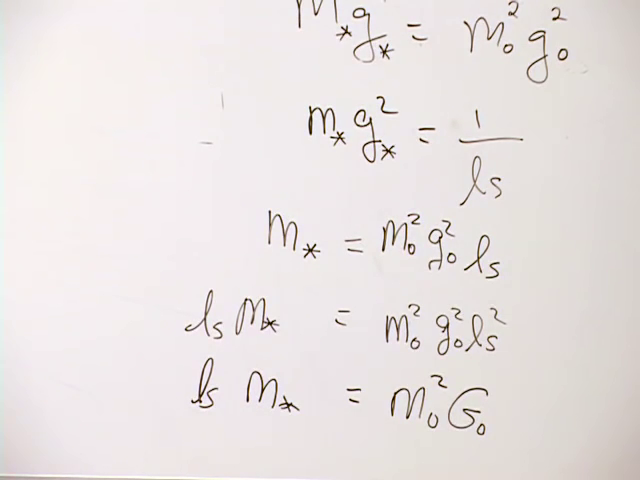
\includegraphics[width=0.68\textwidth]{lecture_07_figure_08.png}
\caption{完整的过渡代数，包括 \(M_*\ell_s=M_0^2g_{s,0}^2\ell_s^2=M_0^2G_{N,0}\)。}
\lectureframe{00:54:40.000}
\end{figure}

\begin{classroomqa}
\audiencequestion{当两个曲线方程相除时，\(\ell_s\) 最终应该在分子上还是分母上？\lecturetimestamp{00:52:41}}
\lecturerresponse{分子上。除以 \(1/\ell_s\) 相当于乘以 \(\ell_s\)，这就是为什么 \(M_*\sim M_0^2g_{s,0}^2\ell_s\)。}
\end{classroomqa}

在过渡点处弦公式成立，因此
\begin{equation}
S_*\sim M_*\ell_s.
\end{equation}
熵沿路径保持不变。将此陈述与方程~\eqref{eq:l07-crossover-result} 结合，得到原始目标黑洞的熵：
\begin{equation}
S_{\mathrm{BH}}(M_0)
\sim M_0^2G_{N,0}
\sim M_0^2\ell_{p,0}^2.
\label{eq:l07-final-correspondence}
\end{equation}
这就是所期望的面积律标度。

\section{对应关系证明了什么、没有证明什么}

这一构造并不是说原本强引力黑洞是一条自由弦。它把物体移到弦计数可信的区域，在那里读取熵，并沿可逆路径把该熵带回来。这一过渡是渐变而非位置明确的相边界，因此这一估计无法确定方程~\eqref{eq:l07-bh-exact} 中的系数 \(1/4\)。

尽管如此，同样的逻辑在参数意义上适用于带电黑洞、其他维度中的黑洞物体以及延展的黑膜。更对称和超对称的例子允许受保护的状态计数，在耦合变化时保留精确信息；那些方法能恢复数值系数，但增加了当前概念性论证所不需要的数学工具。

最重要的是，这一计算提供了微观解释。熵是隐藏结构的证据。流体力学描述密度、压强和流动，却省略了分子；流体的熵揭示出这类微观自由度存在。广义相对论同样描述视界而不展示其微观态。弦计数表明，一个自洽的量子引力理论可以包含足够多的态来解释黑洞熵。

\begin{classroomqa}
\audiencequestion{如果 \(S\sim M^3\ell_p^3\) 而不是二次结果，那会意味着什么？\lecturetimestamp{00:59:41}}
\lecturerresponse{那看起来会像体积律。房间里的普通物质或一杯咖啡的熵与体积成正比；二次答案之所以特殊，是因为通过 \(R_s\sim M\ell_p^2\)，它与视界面积成正比。}
\end{classroomqa}

这一结果是贝肯斯坦--霍金熵不仅仅是一种形式上的热力学类比的证据。它指向微观引力自由度，尽管基本推导并未逐个显现这些自由度。

\section{从最大熵到全息}

我们现在改变问题。不再询问指定状态的熵，而是询问与一个区域相容的最大熵。

从房间的普通点阵模型开始。将体积划分为大小为\(V_{\mathrm{cell}}\)的元胞，并让每个元胞携带一个是非问题：被占据还是空着。Susskind给这个假想原子起了一个故意荒谬的名字``meatonium''，以免任何现实的原子细节分散对计数的注意力。如果
\begin{equation}
N=\frac{V}{V_{\mathrm{cell}}},
\end{equation}
那么构型数和最大熵为
\begin{equation}
\Omega=2^N,
\qquad
S_{\max}=\log\Omega=N\log2
\sim\frac{V}{V_{\mathrm{cell}}}.
\label{eq:l07-volume-count}
\end{equation}

\begin{figure}[htbp]
\centering
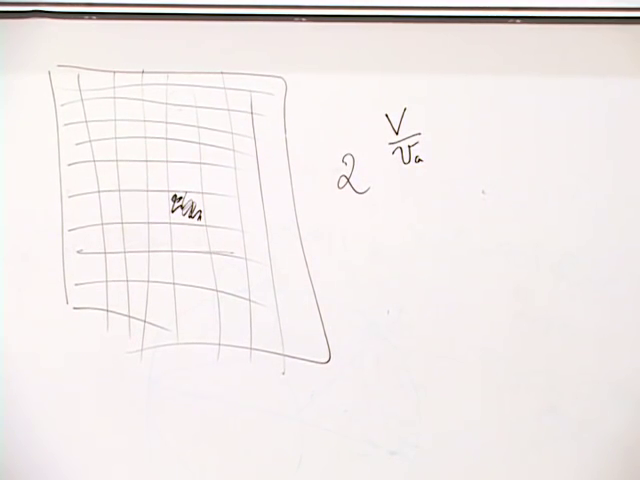
\includegraphics[width=0.68\textwidth]{lecture_07_figure_09.png}
\caption{房间被划分为元胞，每个元胞有两个状态。这计数的是最大熵，而不是班级所在的有序房间的熵。}
\lectureframe{01:05:20.000}
\end{figure}

实际房间远低于这个最大值。一个混沌地探索所有这些元胞选择的状态会极其炽热。从玩具模型中保留下来的是普通预期：独立自由度的数目，因而最大熵，随体积标度。

引力推翻了这一预期。考虑一个球形区域，其边界面积为\(A\)，初始熵为\(S_{\mathrm{i}}\)，质量为\(M\)，且小于恰好填满该球的黑洞质量\(M_{\mathrm{BH}}\)。如果\(M\)更大，其视界就已经延伸到所选边界之外。

现在送入一个质量为\(M_{\mathrm{BH}}-M\)的壳层。其组成无关紧要；讲座允许光、普通物质，甚至瑞士奶酪。安排它坍缩。最终状态是一个黑洞，其视界恰好填满该区域，熵为
\begin{equation}
S_{\mathrm{f}}=\frac{A}{4G_N}.
\end{equation}
第二定律要求
\begin{equation}
S_{\mathrm{i}}\le S_{\mathrm{f}}
=\frac{A}{4G_N}.
\label{eq:l07-holographic-bound}
\end{equation}

\begin{figure}[htbp]
\centering
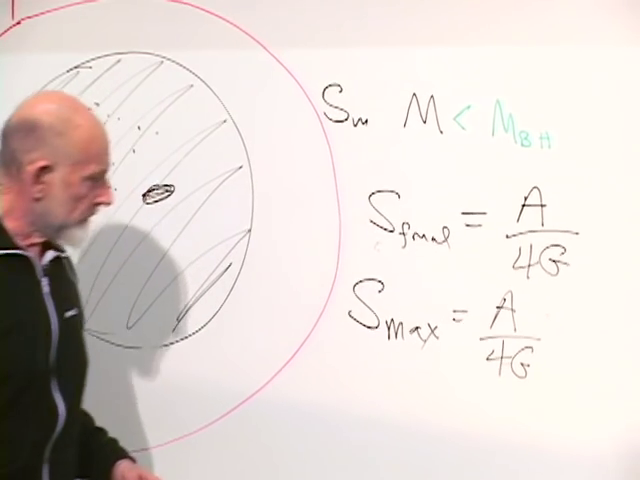
\includegraphics[width=0.70\textwidth]{lecture_07_figure_10.png}

\vspace{0.5em}
\begin{tikzpicture}[scale=0.88]
  \draw[thick] (0,0) circle (1.35);
  \draw[very thick,red!70!black] (0,0) circle (2.05);
  \fill[gray!25] (0,0) circle (1.32);
  \node at (0,0) {\(M,S_{\mathrm{i}}\)};
  \draw[-{Latex[length=3mm]},thick,red!70!black] (3.5,0)--(2.15,0);
  \node[align=center,right] at (3.5,0) {incoming shell\\\(M_{\mathrm{BH}}-M\)};
  \node[below] at (0,-2.2) {final horizon area \(A\)};
\end{tikzpicture}
\caption{壳层构造。足够的额外质量被向内送入，以形成一个视界恰好填满所选区域的黑洞。}
\lectureframe{01:13:30.000}
\end{figure}

因为该大小的黑洞是一个允许的状态并使不等式饱和，所以最大熵为
\begin{equation}
S_{\max}=\frac{A}{4G_N}.
\label{eq:l07-holographic-maximum}
\end{equation}
这就是计数形式的全息原理：引力区域中独立自由度的最大数目随其边界的面积标度，大约每个普朗克面积一个量级为一的自由度，而不是随内部普朗克体积的数目标度。\editorialnote{壳层论证假设该区域能够以所述方式被包围并坍缩。更一般的时空需要协变熵界，但球形论证捕捉了讲座中所用的原理。}

这种差异是巨大的。局域场论直觉表明，在不同内部点作出的选择应当独立组合，产生体积律。引力说，足够多的此类选择本身就会坍缩，而黑洞提供了更大的容许熵。因此，边界计数不是对体积计数的微小修正；它是希尔伯特空间的一种不同组织方式。

\begin{classroomqa}
\audiencequestion{对于一个密度大致均匀的极大宇宙，会发生什么？\lecturetimestamp{01:15:48}}
\lecturerresponse{这个问题需要宇宙学，而不是静态球形构造。它促使我们立即转向爱因斯坦方程的膨胀解。}
\end{classroomqa}

\begin{classroomqa}
\audiencequestion{面积界与不确定性原理有关吗？\lecturetimestamp{01:16:03}}
\lecturerresponse{讲座将这个问题留作开放，接下来转向宇宙学。}
\end{classroomqa}

\section{膨胀的空间}

我们在此不会从爱因斯坦方程推导宇宙学解；我们将写出这些解并学习如何解读它们。空间切片可以是正曲率且闭合的、负曲率且双曲的，或平坦的。就目前的讨论而言，取依赖于时间的时空中的空间平坦欧几里得切片。

\begin{classroomqa}
\audiencequestion{普通欧几里得空间的时空类似物是什么？\lecturetimestamp{01:19:37}}
\lecturerresponse{闵可夫斯基空间。这里考虑的宇宙学具有平坦空间切片，但不是闵可夫斯基时空，因为其空间度规随时间变化。}
\end{classroomqa}

熟悉的氣球圖像描述的是一個低一維的閉合膨脹曲面。Susskind 回憶曾用一個畫有標記的大氣球嘗試演示；記號筆削弱了橡膠，結果真的發出一聲爆響。這次意外也暴露了該類比中的一個概念缺陷。當普通氣球膨脹時，其橡膠分子彼此分離，材料變薄直至破裂。宇宙學空間並不會獲得被稀釋的局部定律。為保留該類比，必須想像不斷插入新的橡膠分子，使每個小塊都保持相同的局部性質。在平坦模型中，則將氣球換成一張被均勻向外拉伸並同樣得到補充的大薄片。

在數學上，膨脹體現在度規中：
\begin{equation}
\begin{aligned}
ds^2&=-dt^2+a(t)^2d\mathbf{x}^2,\\
d\mathbf{x}^2&=\delta_{ij}\,dx^i dx^j
=dx^2+dy^2+dz^2.
\end{aligned}
\label{eq:l07-frw-metric}
\end{equation}

\begin{figure}[htbp]
\centering
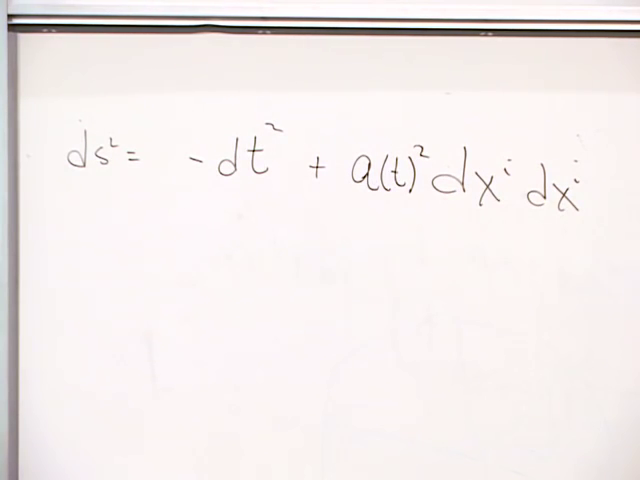
\includegraphics[width=0.72\textwidth]{lecture_07_figure_11.png}
\caption{黑板上寫出的空間平坦膨脹度規。}
\lectureframe{01:25:10.000}
\end{figure}

保持空間坐標固定的點稱為共動點。若兩個這樣的點具有坐標間隔 \(\Delta x\)，則它們在時刻 \(t\) 的固有距離為
\begin{equation}
D(t)=a(t)\Delta x.
\label{eq:l07-proper-distance}
\end{equation}
它們的坐標不動，但二者之間的度規距離發生變化。在固定 \(\Delta x\) 下求導，
\begin{equation}
V=\dot D=\dot a\,\Delta x
=\frac{\dot a}{a}D.
\end{equation}
定義哈勃參數
\begin{equation}
H(t)=\frac{\dot a(t)}{a(t)}.
\label{eq:l07-hubble-parameter}
\end{equation}
於是
\begin{equation}
V=H(t)D,
\label{eq:l07-hubble-law}
\end{equation}
這就是在固定宇宙時刻的哈勃定律。

\begin{figure}[htbp]
\centering
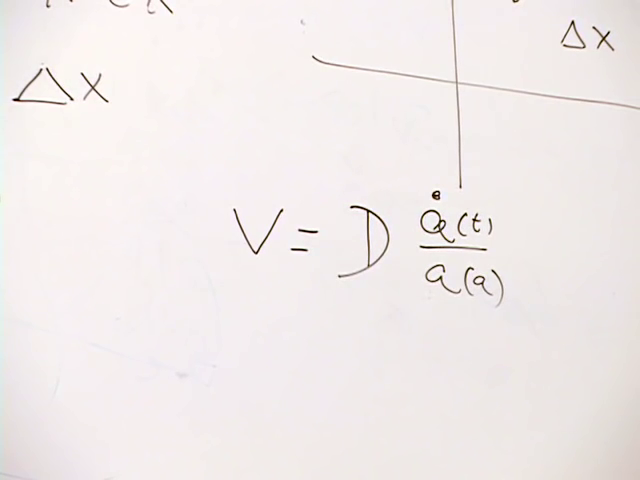
\includegraphics[width=0.68\textwidth]{lecture_07_figure_12.png}
\caption{黑板上寫出的等時退行定律：\(V=D\,\dot a/a\)。}
\lectureframe{01:29:10.000}
\end{figure}

``哈勃常數''這一名稱可能引起誤解。一般而言，\(H(t)\) 隨時間變化。真正在空間上恆定的是同一時間切片上每一對共動點的比值 \(V/D\)。

\begin{classroomqa}
\audiencequestion{對於遙遠星系，在此關係中出現的是哪個時刻？我們是在更早的時期觀測到它們的。\lecturetimestamp{01:31:10}}
\lecturerresponse{式~\eqref{eq:l07-hubble-law}是一個等時陳述。觀測沿著一條指向過去的光線進行，並在更早的時刻對遙遠星系取樣，因此測得的紅移與距離之間的關係需要完整的光錐歷史，而不是 \(H\) 的某一個瞬時值。}
\end{classroomqa}

\begin{figure}[htbp]
\centering
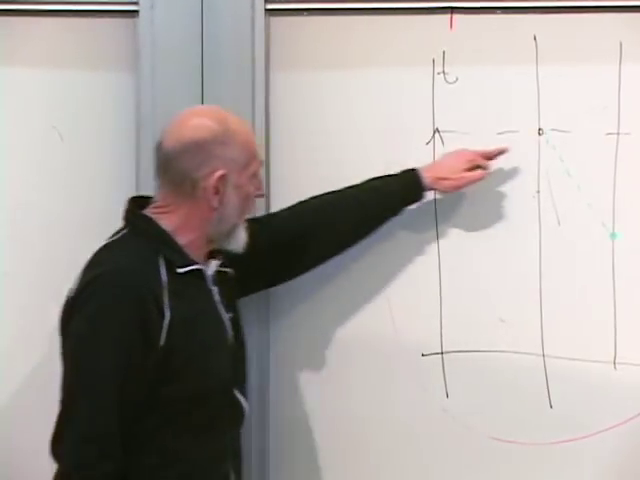
\includegraphics[width=0.66\textwidth]{lecture_07_figure_13.png}
\caption{用於區分等時間隔與觀測者沿過去光線所見的時空示意圖。}
\lectureframe{01:33:20.000}
\end{figure}

\section{哈勃尺度與德西特膨脹}

在單位 \(c=1\) 下，式~\eqref{eq:l07-hubble-law}給出退行速率為 1 的距離
\begin{equation}
D_H=\frac{1}{H}.
\label{eq:l07-hubble-radius}
\end{equation}
更遙遠的共動點可以有 \(V>1\)，甚至 \(V\gg1\)，而不違反狹義相對論。它們並非以超光速經過局部觀測者；它們的固有間隔增大，是因為其間的幾何本身在膨脹。\editorialnote{對於一般的隨時間變化的宇宙學，\(1/H\) 是哈勃半徑，並不自動是事件視界。在接下來討論的德西特情形中，它成為恆定的視界尺度。}

在許多較早的減速宇宙學模型中，\(H(t)\) 減小，而 \(1/H(t)\) 增大，因此曾經以超光速退行的區域後來可以進入因果接觸。講座中討論的晚期圖像則趨近於一個正常數 \(H\)。此時 \(1/H\) 保持固定，膨脹方程變為
\begin{equation}
\frac{\dot a}{a}=H,
\qquad
\dot a=Ha.
\label{eq:l07-constant-h}
\end{equation}

\begin{classroomqa}
\audiencequestion{恆定的哈勃參數的單位是什麼？\lecturetimestamp{01:38:24}}
\lecturerresponse{時間的倒數。等價地，取 \(c=1\) 時，它是長度的倒數。量 \(H^{-1}\) 同時提供了一個膨脹時間和一個距離尺度；講座使用了大約一百五十億年的數量級例子。}
\end{classroomqa}

式~\eqref{eq:l07-constant-h}的解為
\begin{equation}
a(t)=a_0e^{Ht}.
\label{eq:l07-desitter-scale-factor}
\end{equation}

\begin{classroomqa}
\audiencequestion{什麼函數的變化率與自身成正比？\lecturetimestamp{01:39:04}}
\lecturerresponse{指數函數。因此標度因子為 \(a_0e^{Ht}\)，而度規中的空間係數 \(a(t)^2\) 按 \(e^{2Ht}\) 增長。}
\end{classroomqa}

\begin{figure}[htbp]
\centering
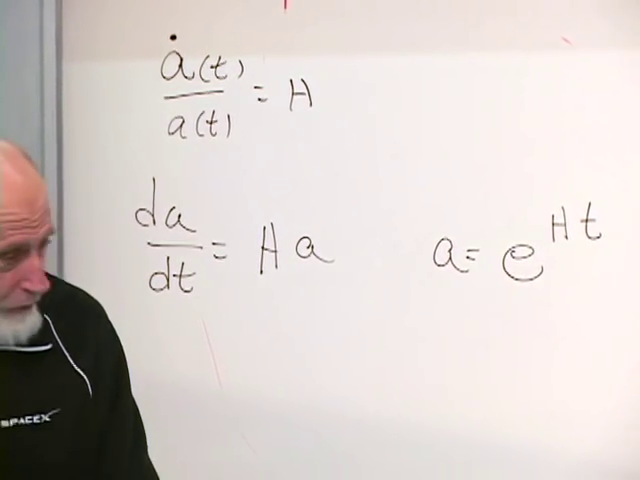
\includegraphics[width=0.70\textwidth]{lecture_07_figure_14.png}
\caption{黑板上寫出的常 \(H\) 方程及其指數解。}
\lectureframe{01:39:30.000}
\end{figure}

具有這種指數膨脹的時空是德西特空間。其恆定的哈勃尺度在有限固有距離處產生一個事件視界。該幾何在某種意義上是黑洞圖像的互補：觀測者始終處於一個宇宙學視界之內，而足夠遙遠的物體退行，永遠無法發出信號追上該觀測者。黑洞視界對外部觀測者隱藏內部；德西特視界則對觀測者隱藏其可及區域的外部。與普通蒸發黑洞不同，這裡將理想的德西特幾何視為持續存在。這一比較才剛剛開始。下一講將展開視界、其熱力學以及它為宇宙學帶來的種種疑難。